% Loader dokumentklassen revtex4. S�tter sproget i dokumentet til dansk, papirtypen til A4, laver to s�jler og siger at vi gerne vil bruge matematikpakkerne fra ams.
\documentclass[a4paper,onecolumn,amsmath,amssymb]{revtex4-1}
\usepackage[english]{babel}%Giver mulighed for dansk orddeling. Slet kun hvis du VED hvad du laver, eller skal skrive noget på engelsk.
\usepackage[latin1]{inputenc}	%Tillader danske tegn
\usepackage[T1]{fontenc}	%Tillader danske tegn
\usepackage{graphicx}		%Tillader inds�ttelse af billeder
\usepackage{dcolumn}		%Bruges til at lave matematiske tabelsøjler... se datatabel
\usepackage{booktabs}		%linjer i tabeller...
\usepackage{mathtools}		%Ekstra matematik... bare lad den være, du får muligvis brug for den.
\usepackage{xcolor}
\usepackage{epsfig}
\usepackage{amssymb}
\normalsize
%siunitx-pakken er ny ift. den originale template, s� der henvises i tekstan til en anden pakke, beklager.
\usepackage{siunitx}	%Bruges \SI{<tal>}{<enhed>}, \si{<enhed>} eller \num{<tal>}.
\sisetup{output-decimal-marker={.},separate-uncertainty=true}%Sørger for komma som decimalmark�r. Virker også ved decimaltal, hvis man bruger \num{<tal>}.
\usepackage{url}		 %bruges til at formattere url'er... kan sagtens udelades.
%Det f�lgende laver to makroer, \tref{} og \fref, der kan bruges ligesom \ref til at referere til hhv. tabeller og figurer. 
%De inds�tter selv ordet Tabel/Figur, og s�rger for at der ikke sker et linjebrud mellem dette og nummeret.
\newcommand{\tref}[1]{\tablename~\ref{#1}}
\newcommand{\fref}[1]{\figurename~\ref{#1}}
%Tilsvarende for ligninger. Indsætter "ligning (#)".
\newcommand{\lref}[1]{ligning~\eqref{#1}}
	% \eqref laver en reference med parenteser omkring (til brug ved ligninger.)
\usepackage[margin=1.0in]{geometry}
%Disse makroer indsætter ordene "PicoScope" og "EasyPlot" i teksten (med store bogstaver. Husk at sætte "{}" bagefter for at få et mellemrum.
%Jeg har lavet dem fordi jeg blev træt af at sidde og trykke shift hele tiden, og for at få det til at st� ens. Brug dem, eller lad være.
\newcommand{\picos}[0]{\textsc{PicoScope}} %hedder \picos for ikke at komme i kambolage med pico fra SIunits.
\newcommand{\epw}[0]{\textsc{EasyPlot}}    %epw er navnet på programfilen for easyplot, men det har ingen betydning for makroen. Jeg valgte det fordi det var noget jeg kunne huske, og det kan sagtens ændres.
\newcommand{\matl}[0]{\textsc{Matlab}} %Skriver Matlab med small caps.

%hyperref-pakken kan bruges til at redigere pdf-metadata. Det kan v�re et nice touch, men er generelt ikke påkrævet. Laver automatisk referencer i teksten til farvede hyperlinks i.
\usepackage{amsmath,amssymb}
\usepackage{hyperref}
\usepackage{subcaption}
\usepackage{verbatim}
\usepackage{atbegshi} %%Removes blank page before title page
\AtBeginDocument{\AtBeginShipoutNext{\AtBeginShipoutDiscard}}



\hypersetup
{   pdfsubject={Rapport},
	pdfauthor={}
    pdftitle={Draft Thesis},
    pdfstartview=FitH,
    colorlinks=true}
    \usepackage{titlesec}

\titleformat*{\section}{\LARGE\bfseries}
\titleformat*{\subsection}{\Large\bfseries}
\titleformat*{\subsubsection}{\large\bfseries}
\titleformat*{\paragraph}{\large\bfseries}
\titleformat*{\subparagraph}{\large\bfseries}
    
%F�lgende gør, at subscripts bliver ikke-kursiv. Anvendes X_|<subscript>|. Erstattes evt. med X_{\mathrm{<subscript>}}.
\makeatletter
\begingroup
\catcode`\_=\active
\protected\gdef_{\@ifnextchar|\subtextup\sb}
\endgroup
\def\subtextup|#1|{\sb{\textup{#1}}}
\AtBeginDocument{\catcode`\_=12 \mathcode`\_=32768 }
\makeatother
\usepackage{graphicx}
\usepackage{placeins}
\usepackage[danish=quotes]{csquotes} %Danske citationstegn. \enquote{}
\usepackage{bbm}

%Lad disse to linjer v�re. De s�rger for at bunden af siden bliver p�n, og fjerner indryk ved afsnit.
\raggedbottom
\parindent = 5pt
\renewcommand{\thesection}{\arabic{section}}
 \renewcommand{\thesubsection}{\thesection.\arabic{subsection}}
 \renewcommand{\thesubsubsection}{\thesubsection.\arabic{subsubsection}}
 
\newcommand{\incomplete}{\textcolor{red}{\large NOT DONE YET!}}
\newcommand{\noncorr}{\textcolor{red}{\Large NOT CORRECTED YET!}} 
\newcommand{\missing}{\textcolor{red}{\large SOME MATERIAL IS MISSING HERE}}
\newcommand{\scatrat}{a_{AB}/a_{AA}}
\newcommand{\massrat}{m_{A}/m_{B}}
\newcommand{\invarat}{a_{AA}/a_{AB}}
\newcommand{\sgn}{\textrm{sgn}}

\usepackage{soul,color}
%\usepackage{refcheck}
\begin{document}
%Dette er boksen i toppen. Lad den v�re.
%\framebox[\textwidth][l]{\textbf{
%\begin{tabular}{p{\linewidth}l}
%Modtaget dato:  & {Godkendt:}\\
%& Dato:\\
%& Underskrift:\\
%(forbeholdt instruktor) & \\
%\end{tabular}
%}}
%Boksen slutter her.

%\bigskip
%\title{Kursus i eksperimentelle øvelser, øvelse 4: Rutherfordspredning med 400 kV van de Graaff
%accelerator.}

\
 %Hvis begge personer studerer det samme sted, kan informationen her flyttes til \affiliation
%Forfatter 2 
 %Det er nok de f�rreste der er s� priviligerede at have holdnummer pi, s� skift denne tekst ud
	% Bem�rk at det har betydning hvor \affilliation og \altaffiliation er placeret i forhold til \author. De virker p� alle forfattere der kommer f�r dem.


\begin{titlepage}
\pagenumbering{gobble}
%\title{\Huge{Properties of Three-Body Systems with Varying Pairwise Interactions}}
\vspace{1cm}
%\author{Jens C. Therkildsen\\
%Aarhus University\\
%Insitute of Physics and Astronomy}
%%\date{August, 2016}
%\vspace{10cm}
\title{\Huge{Intro to ACA Lab project, 2018.}}
\author{Jens C. Therkildsen,  Jonathan Brandtjensen\\
Aarhus University\\
IFA}
\maketitle
\end{titlepage}
\newpage
\pagenumbering{gobble}
\mbox{}
\newpage
\pagenumbering{roman}

\tableofcontents

\cleardoublepage

\pagenumbering{arabic}


\noindent
\section{\textbf{Introduction}}

For our project, we decided to attempt to implement a automatic parking corrector, specifically for packing between objects. The main feature which has been implemented, is that when an object is detected within a vicinity $\kappa$, but larger than a vicinity $\ell_{min}$, of either end of a small car, the car will automatically move itself towards the object and stop at a distance $\ell_{min}$ from it. This is done through a ultrasonic distance sensor on both ends of the car. This creates the basis for expanding the project to include two objects, and making the car find the midpoint, as the routine employed is the same, the difference being delay and system effects introduced by having more inputs going into the system at the same time.\\


We keep the system to first order, not considering integrators within implemented control schemes, as the only differentiated quantity is the speed, $v_0$, which is constant most of the time,  leaving us only to consider the relative distances, even allowing neglection of the length of the car for now. 

\section{\textbf{Overview of Scenarios}}

The left-right symmetry of the problem eliminates half of our cases instantly. The largest disctinction between all cases is whether or not one or two objects are involved. However only the case involving a single object will be discussed in the report.\\
\subsection{\textbf{One  Object}}
\begin{figure}
	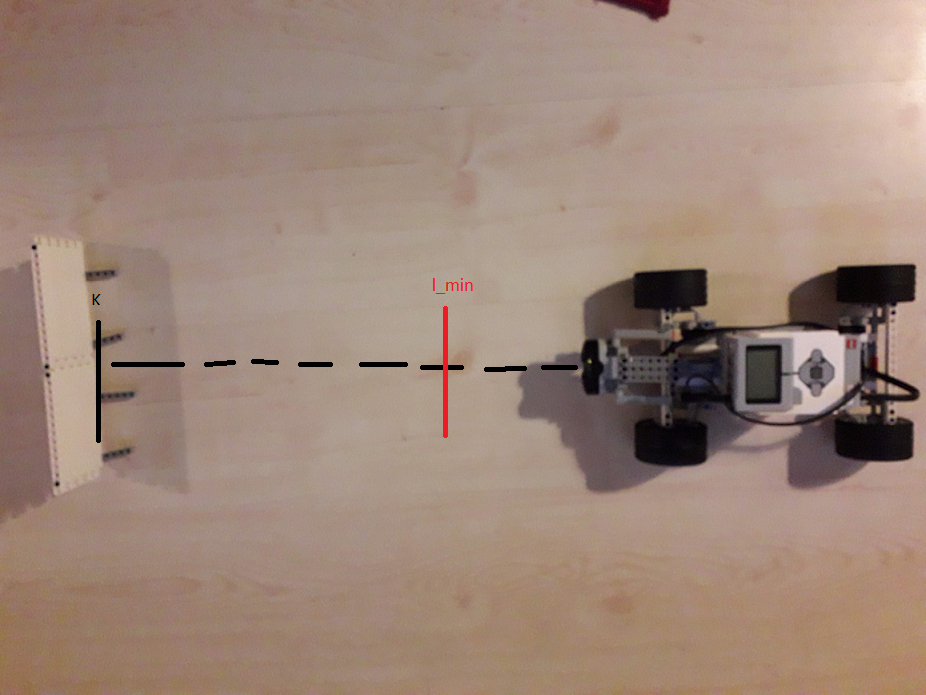
\includegraphics[width=\textwidth]{useCase1.png}
	\caption{\textit{Picture showing car detecting object K, before needed to move until K is within distance $\ell_{min}$ }\label{fig:usecase1picture}}
\end{figure}
\FloatBarrier

In the primary use case, a single object is detected with the distance K from the sensor. After comparing whether K is within the $\ell_{min}$ distance, the car will  move either forward or backwards to maintain a distance of $\ell_{min}$ to the object. In the case of \ref{fig:usecase1picture} the would move forward.

\section{\textbf{ Hardware Considerations and Physical Set Up }}
\subsection{\textbf{Sensor}}
For the project, we had two sensors to choose between: The EV3 Infra-red and the EV3 Ultrasound sensor. We ended up selecting the ultrasound sensor following a the measurements and considerations mentioned hereafter.\\
For our purposes, we had some straightforward of requirements for our sensor:
\begin{enumerate}
\item We require the sensor to be able to consistently provide measurements to some accuracy (this accuracy in turn determining $\ell_{min}$) and for the accuracy, and the measurements, to be stable.
\item The sensor readings must be unmolested by the physical surroundings, as might be the case with objects on the perimeter of sensors field of view.
\item The time delay between the movements of an object whose proximity is being recorded, and the sensor outputting this new position, must be fairly small. This is important, as it imposes a constraint on the movement speed of our car, $v_0$.
\end{enumerate}

Having carried out a series of tests on each of the sensors we ended up settling on the EV3 Ultrasound sensor, as this was the one best fulfilling the needs outlined in the points above. Based on these tests were able to determine values for the parameters mentioned in the above points. The parameters set is provided in the section on modelling.
\subsection{\textbf{DC Motor}}
In this project a Lego EV3 DC Motor is used. Considerations, such as those described in the subsection on sensors, were not needed here as there were not really any other obvious options on the table.\\

The EV3 DC motor works as any other DC motor, and is therefore in principal already self-regulating by virtue of the induced e.m.f being proportional to the motor speed. However, this regulation would primarily be in response to a change in load (such as the chassis and wheels of the car).
\section{\textbf{The system and it's transfer function}}
\subsection{\textbf{Modelling, Parameters and Maths}}
A primary ingredient in the modelling of this system is to determine a transfer function for the DC engine which provides a suitable balance between described complexity and accuracy.\\ 

Below is a simplified schematic diagram depicting the inside of the DC motor:\\

\FloatBarrier
\begin{figure}
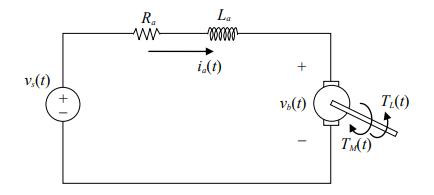
\includegraphics[width=\textwidth]{DCMotor_with_load.png}
\caption{\textit{Schematic drawing of a DC engine with a payload (in our case, the chassis of the LEGO car. The quantity $v_s (t)$ is the input voltage, $i_a (t)$ is armature current, $v_b(t)$ is the induced back e.m.f, $R_a$ is the armature resistance and $L_a$ is the inductance of the motor coil. Finally, $T_M (t)$ is the torque generated by the motor and $T_L $ is the torque of the load counteracting the torque generated by the motor, as well as friction }\label{fig:dcmotorwithload}}
\end{figure}
\FloatBarrier

The first of the differential equations describing the system is obtained through use of Kirchhoff's second voltage law and the fact that the back e.m.f, $v_b (t)$, is directly proportional to the angular velocity of the rotor (the shaft) in the motor, i.e., $v_b (t)=k_b * \omega (t)$, where the proportionality constant $k_b$ is the "back e.m.f" constant. \\

The next of the two differential equations describing the system is obtained by considering Newton's laws in terms of moments of inertia and torque (as seen in figure \ref{fig:dcmotorwithload}). Further simplification of the resulting equations can be done by considering the system in it's steady state.\\

In steady state we have that $v_b (t) =v_s (t)$, and therefore $\omega (t)=\omega$, i.e., constant. In steady state the same is also true of the current $i_a (t)$, the motor torque $T_M $ and the input voltage $v_s$. Considering the power input in the system, and that it must balance with the sum of the output and what is dissipated  in the resistor, and keeping in mind that the motor torque $T_M$ is directly proportional to the current $i_a$, then it can be seen that the proportionality constant between torque and current is identical to the previously mentioned proportionality back e.m.f constant $k_b$.\\

These considerations then produce the two differential equations describing the system.\\

The mechanical one:\\

\begin{equation}
J_M\frac{d\omega(t)}{dt}+B_M\omega(t)=T_M (t)-T_L (t)
\end{equation}

The electrical one:\\

\begin{equation}
L_a\frac{d i_a (t)}{dt}+R_a i_a+k\omega (t)=v_s (t)
\end{equation}

Recalling that $T_L(t)$ is the load on the vehicle (e.g., it's mass and the friction between wheels and road), it can be considered approximately constant, so we can for all purposes ignore it and consider it as falling under $T_M(t)$ . Using this,and that one can write $T_M(t)=k i_a(t)$, the mechanical equation becomes:\\

\begin{equation}
J_M\frac{d i_a(t)}{dt}+B_M\omega(t) =k i_a (t)
\end{equation}

Applying the Laplace transform, then renders the following mechanical equation:\\
\begin{equation}
 s \left( s J_M + B_M\right)\Theta (s)=k I_a(s)
\end{equation}
With the following electrical equation:\\
\begin{equation}
\left( L_a s+R_a\right)I_a(s)=V_s(s) - k s \Theta(s)
\end{equation}

In the case with which we are concerned we are considering distances rather than velocities, both of these being directly related to the angle and angular velocities by the radius. The output of our DC motor is a measurement of angular velocity this means it is necessary to integrate in any case, and therefore define the angle as output, $\Theta(s)=Y(s)$, and the input voltage as input $V(s)=U(s)$.\\

In what follows subscripts are no longer needed and therefore omitted. Since \\
\begin{equation}
I(s)=\frac{s\left(sJ+B\right)\Theta(s)}{k}=\frac{V(s)-ks\Theta(s)}{L s +R},
\end{equation}
then some rearrangement gives the following transfer function
\begin{equation}
H(s)=\frac{Y(s)}{U(s)}=\frac{\Theta(s)}{V(s)}=\frac{k}{s(sJ+B)(Ls+R)+k^2s}=\frac{k}{s\left((Js+B)(Ls+R)+k^2\right)}.
\end{equation}
This transfer function represents, as it stands above, a second order system. From some internet research, one can see that in DC engines, one will commonly have $\mathcal{O}(R)=10^{-1}$,$\mathcal{O}(L)=10^{-3}$, $\mathcal{O}(J)=10^{-4}$,$\mathcal{O}(k)=10^{-2}$ and $\mathcal{O}(B)=10^{-4}$ in S.I units. The large differences in $\mathcal{O}(R)$ and $\mathcal{O}(L)$ then mean that the pole (s) in the term $(Ls+R)$ must be at least an order or two larger in magnitude than the other from the $(Js+B)$ term. Therefore it can be ignored, as $s$ is exponentiated, and the exponential will therefore die out far more quickly for this pole, making it's overall effects on transient behaviour less significant.\\

In some regards this is not surprising, as the neglected pole represents an electronic term and electronic systems operate on significantly smaller time scales than electronic ones. However, because of this the transfer function of the system then becomes
\begin{equation}
H(s)=\frac{k}{s\left(Js+B+k^2\right)}=\frac{K}{s\left(s\tau+1\right)},
\end{equation}
with the last equation arising by redefining the constants in the first equality to $J=\frac{k\tau}{K}$ and $B=k(\frac{1}{K}-k)$.Although the former is closer to the pole placement that will occur in the next subsection, the latter is more manageable.\\
\subsection{\textbf{Pole Placement}}
To make the transient behaviour of the system as we desire, we can place its poles. It is common practice to treat all systems of second order or higher as a second order system, with the desired system properties being related to a second order transfer function as below\\
\begin{equation}
Q(s)=\frac{\omega_n^2 }{s^2+2\zeta \omega_n ^2 s +\omega_n ^2 }~~.
\end{equation}
Here the damping ration $\zeta=\frac{-ln(\frac{O.S_{\%}}{100})}{\sqrt{\pi ^2 +ln^2(\frac{O.S_{\%}}{100})}}$, where $O.S_{\%}$ is the desired overshoot in percent. Also the settling time $T_s=\frac{4 }{\zeta\omega_n}$, where $T_s$ is the settling time in seconds.\\

For our system, we deemed that a settling time of $T_s=0.5s$ and $O.S_{\%}=10$ to be decent values.  From this the standard form second order transfer function we then determined the position of the desired open loop poles, by solving for zero in the denominator of this form, to be\\
\begin{equation}
s_{\text{Desireable}}=-8.00007\pm10.9151 i
\end{equation}
\subsection{\textbf{State Space Model}}
Having previously disclosed the differential equations and transfer function of the system at hand, it is fairly straight forward to represent the system in state-space. Using the standard forms 
\begin{equation}
\dot x=Ax+Bu ,
\end{equation}
and
\begin{equation}
y=Cx+Du~,
\end{equation}
one of the system's state space representations can be found quite readily. Since the system's transfer function $H(s)$ is second order, the derivative on the left hand side of the first control equation will cause the resulting  system matrices to be 3x3's, however this extra dimension contains no non-zero elements and can therefore be ignored. The state space representation, in phase variable form,then becomes
\begin{equation}
\begin{bmatrix}
\dot x \\
\ddot x
\end{bmatrix}
=
\begin{bmatrix}
0 && 1 \\
0 && -\frac{1}{\tau}
\end{bmatrix}
\begin{bmatrix}
x \\ \dot x
\end{bmatrix}
+
\begin{bmatrix}
0\\ 1
\end{bmatrix}
u
\end{equation}
and
\begin{equation}
y=
 \begin{bmatrix}
\frac{K}{\tau}&& 0
\end{bmatrix}
\begin{bmatrix}
x \\ \dot x
\end{bmatrix}
\end{equation}
\subsection{\textbf{Observer and Controller Design}}
In our system we have one entities performing measurements. A ultrasound sensor, providing running measurements of the relative distance between itself and the obstacle.

Based on the idea that the distance measured by the sensor, is technically a position, we have tried to make a observer with controller design to regulate the change in position until we reach the reference $\ell_{min}$.
\section{\textbf{Implementations and Results}}















































































 







 


 

 

 




























\begin{thebibliography}{99}

\end{thebibliography}






\end{document}